%% (Master) Thesis template
% Template version used: v2
%
% Largely adapted from Adrian Nievergelt's template for the ADPS
% (lecture notes) project.

%% We use the memoir class because it offers many easy to use features.
% Template v2 fixes:
% Removed titlepage from options: LaTeX Warning: Unused global option(s): [titlepage].
% Electronic version that does not waste space
\documentclass[11pt,a4paper,openany,oneside]{memoir}
% Printable version that does waste space (but people like it), uncomment for printing
% \documentclass[11pt,a4paper]{memoir}

%% Packages
%% ========

%% LaTeX Font encoding -- DO NOT CHANGE
\usepackage[OT1]{fontenc}

%% Babel provides support for languages.  'english' uses British
%% English hyphenation and text snippets like "Figure" and
%% "Theorem". Use the option 'ngerman' if your document is in German.
%% Use 'american' for American English.  Note that if you change this,
%% the next LaTeX run may show spurious errors.  Simply run it again.
%% If they persist, remove the .aux file and try again.
\usepackage[english]{babel}

%% Input encoding 'utf8'. In some cases you might need 'utf8x' for
%% extra symbols. Not all editors, especially on Windows, are UTF-8
%% capable, so you may want to use 'latin1' instead.
\usepackage[utf8]{inputenc}

%% This changes default fonts for both text and math mode to use Herman Zapfs
%% excellent Palatino font.  Do not change this.
\usepackage[sc]{mathpazo}

%% The AMS-LaTeX extensions for mathematical typesetting.  Do not
%% remove.
\usepackage{amsmath,amssymb,amsfonts,mathrsfs}

%% NTheorem is a reimplementation of the AMS Theorem package. This
%% will allow us to typeset theorems like examples, proofs and
%% similar.  Do not remove.
%% NOTE: Must be loaded AFTER amsmath, or the \qed placement will
%% break
\usepackage[amsmath,thmmarks]{ntheorem}

%% LaTeX' own graphics handling
\usepackage{graphicx}

%% Added to use tikz diagrams
\usepackage{tikz}
\usetikzlibrary{shapes,arrows,positioning}

%% We unfortunately need this for the Rules chapter.  Remove it
%% afterwards; or at least NEVER use its underlining features.
\usepackage{soul}

%% This allows you to add .pdf files. It is used to add the
%% declaration of originality.
\usepackage{pdfpages}

%% Some more packages that you may want to use.  Have a look at the
%% file, and consult the package docs for each.
%% See the TeXed file for more explanations

%% [OPT] Multi-rowed cells in tabulars
%\usepackage{multirow}

%% Make document internal hyperlinks wherever possible. (TOC, references)
%% This MUST be loaded before cleveref
\usepackage[linkcolor=black,colorlinks=true,citecolor=black,filecolor=black]{hyperref}

%% [REC] Intelligent cross reference package. This allows for nice
%% combined references that include the reference and a hint to where
%% to look for it.
%% Template v2: cleveref already recognizes what is being referenced - one does not need to write Fig./Sec.
% \usepackage{varioref}. Capitalization is prefered in CS
\usepackage[capitalise]{cleveref}

%% [OPT] Easily changeable quotes with \enquote{Text}
\usepackage[german=swiss]{csquotes}

%% Template v2: this prevents warning "Package fmtcount Warning: \ordinal already defined use \FCordinal instead. on input line". See https://tex.stackexchange.com/questions/162353/memoir-class-conflict-with-datetime#comment371926_162358
\let\ordinal\relax
%% [REC] Format dates and time depending on locale
\usepackage{datetime}

%% [OPT] Provides a \cancel{} command to stroke through mathematics.
%\usepackage{cancel}

%% [NEED] This allows for additional typesetting tools in mathmode.
%% See its excellent documentation.
\usepackage{mathtools}

%% [ADV] Conditional commands
%\usepackage{ifthen}

%% [OPT] Manual large braces or other delimiters.
%\usepackage{bigdelim, bigstrut}

%% [REC] Alternate vector arrows. Use the command \vv{} to get scaled
%% vector arrows.
\usepackage[h]{esvect}

%% [NEED] Some extensions to tabulars and array environments.
\usepackage{array}

%% [OPT] Postscript support via pstricks graphics package. Very
%% diverse applications.
%\usepackage{pstricks,pst-all}

%% [?] This seems to allow us to define some additional counters.
%\usepackage{etex}

%% [ADV] XY-Pic to typeset some matrix-style graphics
%\usepackage[all]{xy}

%% [OPT] This is needed to generate an index at the end of the
%% document.
%\usepackage{makeidx}

%% [OPT] Fancy package for source code listings.  The template text
%% needs it for some LaTeX snippets; remove/adapt the \lstset when you
%% remove the template content.
\usepackage{listings}
\lstset{language=TeX,basicstyle={\normalfont\ttfamily}}

% Template v2 fixes: this is an old package, microtype is superior + fixes an error
%% [REC] Fancy character protrusion.  Must be loaded after all fonts.
\usepackage[activate]{microtype}
% \usepackage[activate]{pdfcprot}  % causes the compilation error

%% [REC] Nicer tables.  Read the excellent documentation.
\usepackage{booktabs}


%% Our layout configuration.  DO NOT CHANGE.
%% Memoir layout setup

%% NOTE: You are strongly advised not to change any of them unless you
%% know what you are doing.  These settings strongly interact in the
%% final look of the document.

% Dependencies
\usepackage{eth-template/ETHlogo}

% Turn extra space before chapter headings off.
\setlength{\beforechapskip}{0pt}

\nonzeroparskip
\parindent=0pt
\defaultlists

% Chapter style redefinition
\makeatletter

\if@twoside
  \pagestyle{Ruled}
  \copypagestyle{chapter}{Ruled}
\else
  \pagestyle{ruled}
  \copypagestyle{chapter}{ruled}
\fi
\makeoddhead{chapter}{}{}{}
\makeevenhead{chapter}{}{}{}
\makeheadrule{chapter}{\textwidth}{0pt}
\copypagestyle{abstract}{empty}

\makechapterstyle{bianchimod}{%
  \chapterstyle{default}
  \renewcommand*{\chapnamefont}{\normalfont\Large\sffamily}
  \renewcommand*{\chapnumfont}{\normalfont\Large\sffamily}
  \renewcommand*{\printchaptername}{%
    \chapnamefont\centering\@chapapp}
  \renewcommand*{\printchapternum}{\chapnumfont {\thechapter}}
  \renewcommand*{\chaptitlefont}{\normalfont\huge\sffamily}
  \renewcommand*{\printchaptertitle}[1]{%
    \hrule\vskip\onelineskip \centering \chaptitlefont\textbf{\vphantom{gyM}##1}\par}
  \renewcommand*{\afterchaptertitle}{\vskip\onelineskip \hrule\vskip
    \afterchapskip}
  \renewcommand*{\printchapternonum}{%
    \vphantom{\chapnumfont {9}}\afterchapternum}}

% Use the newly defined style
\chapterstyle{bianchimod}

\setsecheadstyle{\Large\bfseries\sffamily}
\setsubsecheadstyle{\large\bfseries\sffamily}
\setsubsubsecheadstyle{\bfseries\sffamily}
\setparaheadstyle{\normalsize\bfseries\sffamily}
\setsubparaheadstyle{\normalsize\itshape\sffamily}
\setsubparaindent{0pt}

% Set captions to a more separated style for clearness
\captionnamefont{\sffamily\bfseries\footnotesize}
\captiontitlefont{\sffamily\footnotesize}
\setlength{\intextsep}{16pt}
\setlength{\belowcaptionskip}{1pt}

% Set section and TOC numbering depth to subsection
\setsecnumdepth{subsection}
\settocdepth{subsection}

%% Titlepage adjustments
\pretitle{\vspace{0pt plus 0.7fill}\begin{center}\HUGE\sffamily\bfseries}
\posttitle{\end{center}\par}
\preauthor{\par\begin{center}\let\and\\\Large\sffamily}
\postauthor{\end{center}}
\predate{\par\begin{center}\Large\sffamily}
\postdate{\end{center}}

\def\@advisors{}
\newcommand{\advisors}[1]{\def\@advisors{#1}}
\def\@department{}
\newcommand{\department}[1]{\def\@department{#1}}
\def\@thesistype{}
\newcommand{\thesistype}[1]{\def\@thesistype{#1}}

\renewcommand{\maketitlehooka}{\noindent\ETHlogo[2in]}

\renewcommand{\maketitlehookb}{\vspace{1in}%
  \par\begin{center}\Large\sffamily\@thesistype\end{center}}

\renewcommand{\maketitlehookd}{%
  \vfill\par
  \begin{flushright}
    \sffamily
    \@advisors\par
    \@department, ETH Z\"urich
  \end{flushright}
}

\checkandfixthelayout

\setlength{\droptitle}{-48pt}

\makeatother

% This defines how theorems should look. Best leave as is.
\theoremstyle{plain}
\setlength\theorempostskipamount{0pt}

%%% Local Variables:
%%% mode: latex
%%% TeX-master: "thesis"
%%% End:


%% Theorem environments.  You will have to adapt this for a German
%% thesis.
%% Theorem-like environments

%% This can be changed according to language. You can comment out the ones you
%% don't need.

\numberwithin{equation}{chapter}

%% German theorems
%\newtheorem{satz}{Satz}[chapter]
%\newtheorem{beispiel}[satz]{Beispiel}
%\newtheorem{bemerkung}[satz]{Bemerkung}
%\newtheorem{korrolar}[satz]{Korrolar}
%\newtheorem{definition}[satz]{Definition}
%\newtheorem{lemma}[satz]{Lemma}
%\newtheorem{proposition}[satz]{Proposition}

%% English variants
\newtheorem{theorem}{Theorem}[chapter]
\newtheorem{example}[theorem]{Example}
\newtheorem{remark}[theorem]{Remark}
\newtheorem{corollary}[theorem]{Corollary}
\newtheorem{definition}[theorem]{Definition}
\newtheorem{lemma}[theorem]{Lemma}
\newtheorem{proposition}[theorem]{Proposition}

%% Proof environment with a small square as a "qed" symbol
\theoremstyle{nonumberplain}
\theorembodyfont{\normalfont}
\theoremsymbol{\ensuremath{\square}}
\newtheorem{proof}{Proof}
%\newtheorem{beweis}{Beweis}


%% Helpful macros.
%% Custom commands
%% ===============

%% Special characters for number sets, e.g. real or complex numbers.
\newcommand{\C}{\mathbb{C}}
\newcommand{\K}{\mathbb{K}}
\newcommand{\N}{\mathbb{N}}
\newcommand{\Q}{\mathbb{Q}}
\newcommand{\R}{\mathbb{R}}
\newcommand{\Z}{\mathbb{Z}}
\newcommand{\X}{\mathbb{X}}

%% Fixed/scaling delimiter examples (see mathtools documentation)
\DeclarePairedDelimiter\abs{\lvert}{\rvert}
\DeclarePairedDelimiter\norm{\lVert}{\rVert}

%% Use the alternative epsilon per default and define the old one as \oldepsilon
\let\oldepsilon\epsilon
\renewcommand{\epsilon}{\ensuremath\varepsilon}

%% Also set the alternate phi as default.
\let\oldphi\phi
\renewcommand{\phi}{\ensuremath{\varphi}}


% Template v2: BibLaTeX with Biber backend are in my opinion best maintainable citation configurations. IEEE style is common in CS.
% Bibliography
\usepackage[
bibstyle=ieee,
citestyle=numeric,
isbn=true,
doi=true,
sorting=none,
url=true,
% defernumbers=true,
bibencoding=utf8,
backend=biber
]{biblatex} %Imports BibLaTeX package
\addbibresource{refs.bib} %Import the bibliography file

%% Document information
%% ====================

\title{Generalizing Browser Extension CookieAudit for Auditing Consent Popups’ GDPR Compliance}
\author{S. Nastaly}
\thesistype{Bachelor's Thesis}
\advisors{Advisors: Prof.\ Dr.\ D. Basin, Dr.\ K.\ Kubicek, A.\ Bouhoula}
\department{Department of Computer Science}
\date{August 28, 2024}

\begin{document}

\frontmatter

%% Title page is autogenerated from document information above.  DO
%% NOT CHANGE.
\begin{titlingpage}
  \calccentering{\unitlength}
  \begin{adjustwidth*}{\unitlength-24pt}{-\unitlength-24pt}
    \maketitle
  \end{adjustwidth*}
\end{titlingpage}

%% The abstract of your thesis.  Edit the file as needed.
\begin{abstract}
  TODO
\end{abstract}


%% TOC with the proper setup, do not change.
\cleartorecto
\tableofcontents
\mainmatter

%% Your real content!
\chapter{Technical and Legal Background}

This chapter presents the technical foundations of browser extension development and the relevant European Union laws for compliance auditing. We provide a general overview here, while the detailed technical implementation of CookieAudit is discussed in \cref{ch:implementation}.

\section{Browser Extensions}
%We implemented CookieAudit as a browser extension.
%To understand the implementation details in \cref{ch:implementation}, we will give an overview of the architecture and implementation of browser extensions.

Browser extensions are programs that can extend or change the functionality of browsers.
They are built using web technologies (JavaScript, HTML, CSS) and can use the APIs provided by the browser.
The APIs of Chromium-based browsers (e.g., Chrome and Edge) overlap in large parts with the APIs of Mozilla's Firefox, while Apple's Safari sometimes differs significantly.
As a result, many extensions can run in several browser environments.

When building browser extensions for Chromium-based browsers, developers have to split up their code according to the specification by Manifest Version 3~\cite{manifestv3}.
In this section, we first explain the different parts of a general browser extension architecture and then detail the challenges posed by Manifest V3.
\cref{fig:extension-architecture} shows a visualization of the building blocks and their interactions.

\begin{figure}
	\centering
	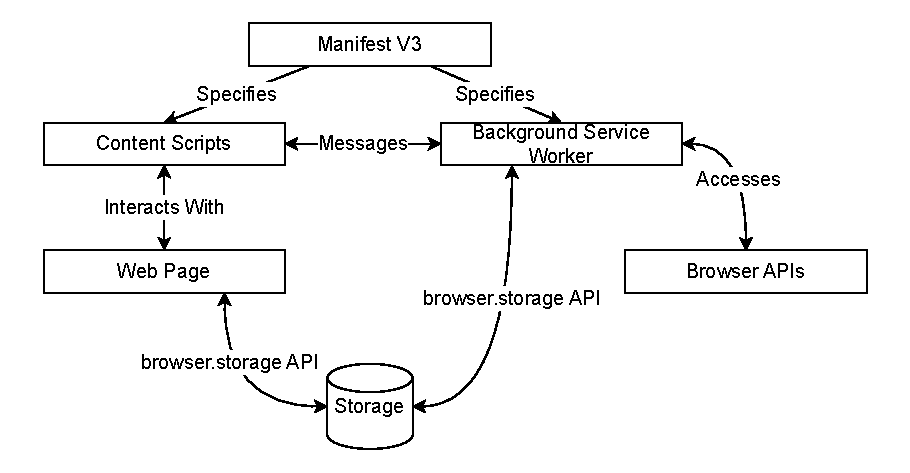
\includegraphics[width=\textwidth]{media/browser-extension-architecture.drawio.pdf}
    \caption{The general architecture of a manifest version 3 browser extension.}
    \label{fig:extension-architecture}
\end{figure}

\subsection{Extension Service Workers} \label{subsec:service-workers}
The Extension Service Worker is the central location for business logic.
By having access to the full WebExtensions API, it is the place to define event listeners,\footnote{
By registering event listeners at the beginning of the service worker, developers can define code that should handle events.
The most relevant events are browser events (e.g., first installation of an extension), tab events (e.g., user navigating to a different URL), and extension events (e.g., messaging between extension components).}
send and receive messages to and from the content scripts and popup
or run time intensive computations~\cite[Ch. 4]{frisbie2023browser}.
Service workers operate asynchronously on a separate thread, preventing interference with website execution. 
They are ephemeral, started by event handlers and terminated when idle.
Therefore, developers must persist important application state to storage (see \cref{subsec:storage}) rather than relying on in-memory variables, as these are reset upon termination.

\subsection{Content Scripts} \label{subsec:content-scripts}
Content scripts are JavaScript programs injected into web pages. 
They can access and modify the page's HTML structure and CSS styles.
By default, content scripts run in an isolated environment, separate from the page's own JavaScript.\footnote{
Developers can deactivate this isolation by setting the execution world to \texttt{MAIN}. Then, the content script will be able to, e.g., read variables of the web page JavaScript.
}
This isolation prevents direct access between the content script and page script.
Variables are not shared, and functions from one context cannot be called by the other.
Content scripts have limited access to the WebExtensions API, for example, they cannot change the current tab's URL.
To interact with the rest of the extension, content scripts use messaging and a shared key-value store.

\subsection{Communication}
Since the extension service worker and the different content scripts run in separate JavaScript environments, variables and functions cannot be accessed across those boundaries.
Instead, browsers provide the messaging API to send and listen for messages.
For example, in the context of cookie notice detection, if a content script has detected a cookie notice and needs to inform the extension service worker about it, one could send a corresponding message as in \cref{fig:message-passing}.

\begin{figure}
	\centering
	\definecolor{backcolour}{rgb}{0.95,0.95,0.92}
	\lstset{backgroundcolor=\color{backcolour}}
	    
	\begin{subfigure}{\textwidth}
		\centering
		\begin{lstlisting}
let response = await chrome.runtime.sendMessage({
  cookieNoticeDetected: true
});
		\end{lstlisting}
		\caption{Sending a message from the content script}
	\end{subfigure}
	    
	\begin{subfigure}{\textwidth}
		\centering
		\begin{lstlisting}
function handleMsg(request,sender,sendResponse) {
  // ... handle message inside request object ...
  // send response to content script:
  sendResponse({ storedData: true });
}
chrome.runtime.onMessage.addListener(handleMsg);
		\end{lstlisting}
		\caption{Handling a message in the background script}
	\end{subfigure}
	    
	\caption{Message passing in Chrome extension}
	\label{fig:message-passing}
\end{figure}

\subsection{Storage} \label{subsec:storage}
Browser extensions often need to be able to store data across browser restarts.
Developers can therefore use the asynchronous\footnote{Even though JavaScript is single-threaded, its asynchronous mechanisms allow non-blocking execution, handling tasks like I/O operations without halting the main thread.} storage API to store key-value pairs serialized as JSON objects. Serializable types include primitives, arrays, and objects\footnote{
Associative arrays, also known as maps or dictionaries, are called objects in JavaScript.
}, but not functions or DOM elements (\texttt{HTMLElement}).

\subsection{Popup}
The primary way for users to interact with a browser extension is through a small dialog called \emph{popup}.
It can only be opened by the user, that is, by clicking the extension’s action icon in the browser toolbar.
Popups are programmed using the same web technologies as websites: HTML, CSS, and JavaScript. 
They have access to all WebExtensions APIs provided by the browser, e.g., storage and messaging. 
\cref{fig:screenshot-popup} shows the popup of CookieAudit.

\begin{figure}
	\centering
	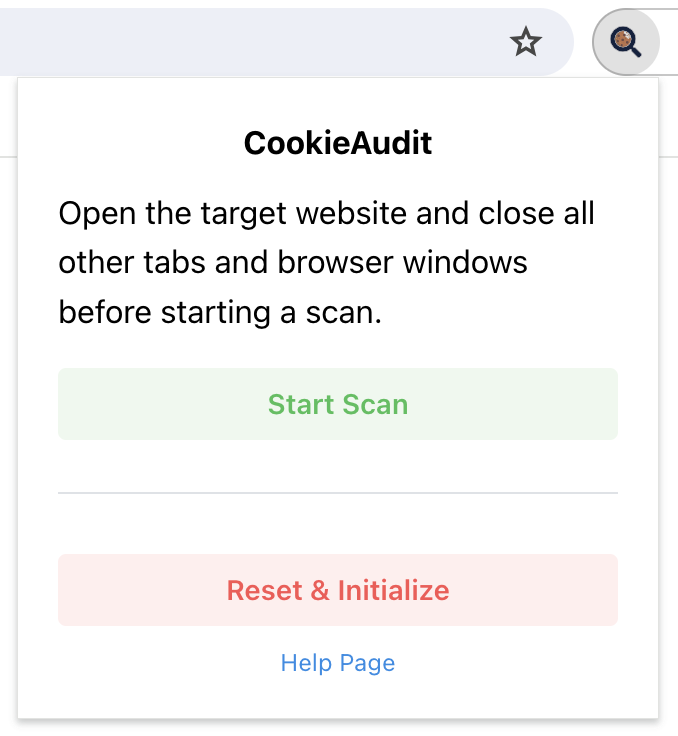
\includegraphics[width=0.5\linewidth]{screenshot_popup.png}
	\caption{Popup dialog of CookieAudit}
	\label{fig:screenshot-popup}
\end{figure}

\subsection{Manifest Version 3} \label{subsec:manifest-v3}
We developed CookieAudit according to Manifest version 3~\cite{manifestv3}.
It is the newest specification of the extensions API for Chromium-based browsers.
Compared to Manifest version 2, it includes API changes and restrictions aimed to increase the security and performance of extensions.
Version 3 has forced some developers to make considerable changes to their extensions~\cite{purdy2024chrome, huczynski2018ublock}, sometimes even reducing the functionality~\cite{hill2024google}.
We present some notable changes between Manifest versions 2 and 3.

\subsubsection{From background scripts to service workers}
In Manifest version 2, developers could use \texttt{background scripts} which effectively were non-visible, persistent web pages.
Many extensions developed for manifest version 2 used the fact that background scripts are never terminated and that their global variables are accessible from the extension popup.
As explained in \cref{subsec:service-workers}, developers cannot rely on those characteristics anymore.
The migration to manifest version 3 sometimes required considerable changes in the architecture of extensions.\footnote{
For example, Gonzalez reported increased complexity following the move of the Bitwarden password manager to Manifest V3~\cite{gonzalez2024bitwarden}.
The switch to service workers made changes in the extension architecture necessary.}
Furthermore, the mechanism requiring idle service workers to restart after being shut down can lead to delays in event handling.
This time to revival can be problematic for time sensitive extensions.

\subsubsection{Execution of arbitrary Strings}
The execution of arbitrary strings with the \texttt{eval()} function could be used for security exploits, as shown by Carlini et al.~\cite{carlini2012evaluation}.
To solve this issue, it is no longer possible to evaluate and execute strings using methods such as \texttt{eval()}, or \texttt{new Function()}.
It is still possible to evaluate and execute WebAssembly,\footnote{WebAssembly is a binary instruction format designed as a fast, safe compilation target for languages like C/C++. It provides JavaScript interoperability and runs in web browsers~\cite{haas2017wasm}.} by specifying \texttt{wasm-unsafe-eval} in the extension manifest.
The ability to run WebAssembly is necessary for many performance critical applications, such as the client-side inference of AI models.

\subsubsection{Other}
Manifest version 3 introduces several other significant changes to browser extension development.
It limits the inspection and modification of live network requests and prohibits the execution of remotely hosted code.\footnote{
All code must be included within the extension package which is published in the extension stores.
}
Furthermore, the new version renames and restructures some WebExtensions API functions.

%\color{orange}
\section{Cookies}
HTTP Cookies are small pieces of text data stored in a user's browser when visiting websites. 
They are initially created by web servers, sent to clients, and stored by browsers. 
Each cookie is associated with a specific domain.
\emph{First-party} cookies are associated with the domain of the website being visited.
For example, when visiting \texttt{news.example}, a cookie may be set with that same domain.
\emph{Third-party} cookies are associated with domains different from the website being visited. 
For instance, if \texttt{news.example} displays an advertisement served from \texttt{ads.example}, the ad server can set cookies with the \texttt{ads.example} domain.
Cookies are automatically sent back to their originating servers with every HTTP request to that domain. 
This adds state to the otherwise stateless nature of HTTP.

Cookies serve various purposes. 
They can provide essential functionality, such as storing user authentication data. 
However, they can also be used to track users across different websites for analytics or advertising purposes.
This is done by creating a unique, identifying key for each user and storing it as a cookie.

\section{General Data Protection Regulation and ePrivacy Directive} \label{sec:legal}
The General Data Protection Regulation (GDPR) and the ePrivacy Directive (ePD) govern data collection and processing in the European Union (EU).
The GDPR defines the data subject (user), controller (typically a website operator), processor (e.g., a cloud provider), and third parties as key entities involved in data collection and processing.
It regulates controllers within the EU as well as those who handle the personal data of EU residents.
Both laws only regulate personal data, which is specifically defined in Article 4 of the GDPR as any information related to an \enquote{identified or identifiable natural person}.
Browser cookies that are not strictly necessary to provide the service, on the other hand, are covered by Article 5(3) of the ePD.
The article requires user consent for storing and accessing data on the users' device, unless strictly necessary for providing a service~\cite{kubicek2024phd}.

For a controller to lawfully process personal data, at least one of the six possible legal bases defined in Article 6 of the GDPR must be satisfied.
These legal bases include consent, contractual necessity, legal obligation, vital interests, public interest, and legitimate interests.
However, in the particular context of websites using personal data and cookies for monetization, only the basis of user consent can be used~\cite{kubicek2024phd}.
Consent must be a \enquote{freely given, specific, informed, and unambiguous indication of the data subject's agreement to the processing of personal data relating to him or her} (Recital 32 of the GDPR).
This implies that consent on websites has to be a voluntary choice by the subject, with equal ease for acceptance and rejection (\emph{freely given}), should always be tailored to a single collection and processing purpose (\emph{specific}), based on clearly communicated practices of data collection and processing (\emph{informed}), and explicitly provided by the user, such as by clicking on a checkbox or signing up for a newsletter (\emph{unambiguous})~\cite{kubicek2024phd}.

Non-compliance with the GDPR can result in severe penalties. 
Supervisory authorities can impose fines of up to €20 million or 4\% of the organization's global annual turnover, whichever is higher~\cite{sanchez_rola2019can}. 

\chapter{Implementation} \label{ch:implementation}

\section{User Interface}
In CookieAudit, users can initiate a website scan, stop it, or download a report summarizing the scan results via the extension popup.
Additionally, CookieAudit displays real-time information about the scan's progress.
For developing the popup's user interface, we chose to use the React JavaScript library.
React offers a declarative programming model that keeps the displayed data synchronized with the underlying data storage.

\section{Cookie Notice Selection}
CookieAudit is designed to automatically analyze and interact with arbitrary cookie notices. 
The initial identification of which HTML element represents the cookie notice could be done either automatically or manually by the user.
Automatic notice selection, e.g., based on heuristics or NLP models, can be error-prone.
On the other hand, a manual selection could provide better accuracy with minimal user effort.
Next, we will give an overview of both approaches and their limitations.

\subsection{Automatic Selection}
Any approach to automated notice selection will always be limited in its accuracy.
For example, Bouhoula et al.~\cite{bouhoula2023automated} achieve a precision of 100\% and a recall of 86.9\%, even though the authors improve in both metrics by building upon the approaches for automatic selection of previous studies.
Those issues fundamentally stem from the many ways of implementing cookie notices in HTML and JavaScript.
Nevertheless, we will present some of those heuristics.

\subsubsection{Crowdsourced Selectors}
HTML elements can be identified with \emph{selectors}. 
Crowdsourced efforts, such as EasyList Cookie~\cite{easylist2024cookie}, maintain lists of cookie notice selectors.
Automated crawlers by Kampanos et al.~\cite{kampanos2021accept} and Bouhoula et al.~\cite{bouhoula2023automated} have used EasyList to find potential cookie notices on websites.

\subsubsection{Stack Level}
The \emph{z-index} is a CSS property of HTML elements that makes elements with a high index appear above elements with a low index. 
Because a user should quickly see a cookie notice, websites usually use a high \emph{z-index} on the notice to let it cover the rest of the website. 
This heuristic has been used by Khandelwal et al.~\cite{khandelwal2023automated} and Bouhoula et al.~\cite{bouhoula2023automated}.

\subsection{User-Aided Selection} \label{subsec:user-aided-selection}
CookieAudit is intended for semi-automated website analysis.
We can therefore rely on user help by using a cookie notice picker tool.
To specify the element containing a notice, users only needs to hover the mouse over it and then confirm the selection. 
An example can be seen in \cref{fig:screenshot-selection}.

\begin{figure}
	\centering
	\begin{minipage}{0.48\textwidth}
		\centering
		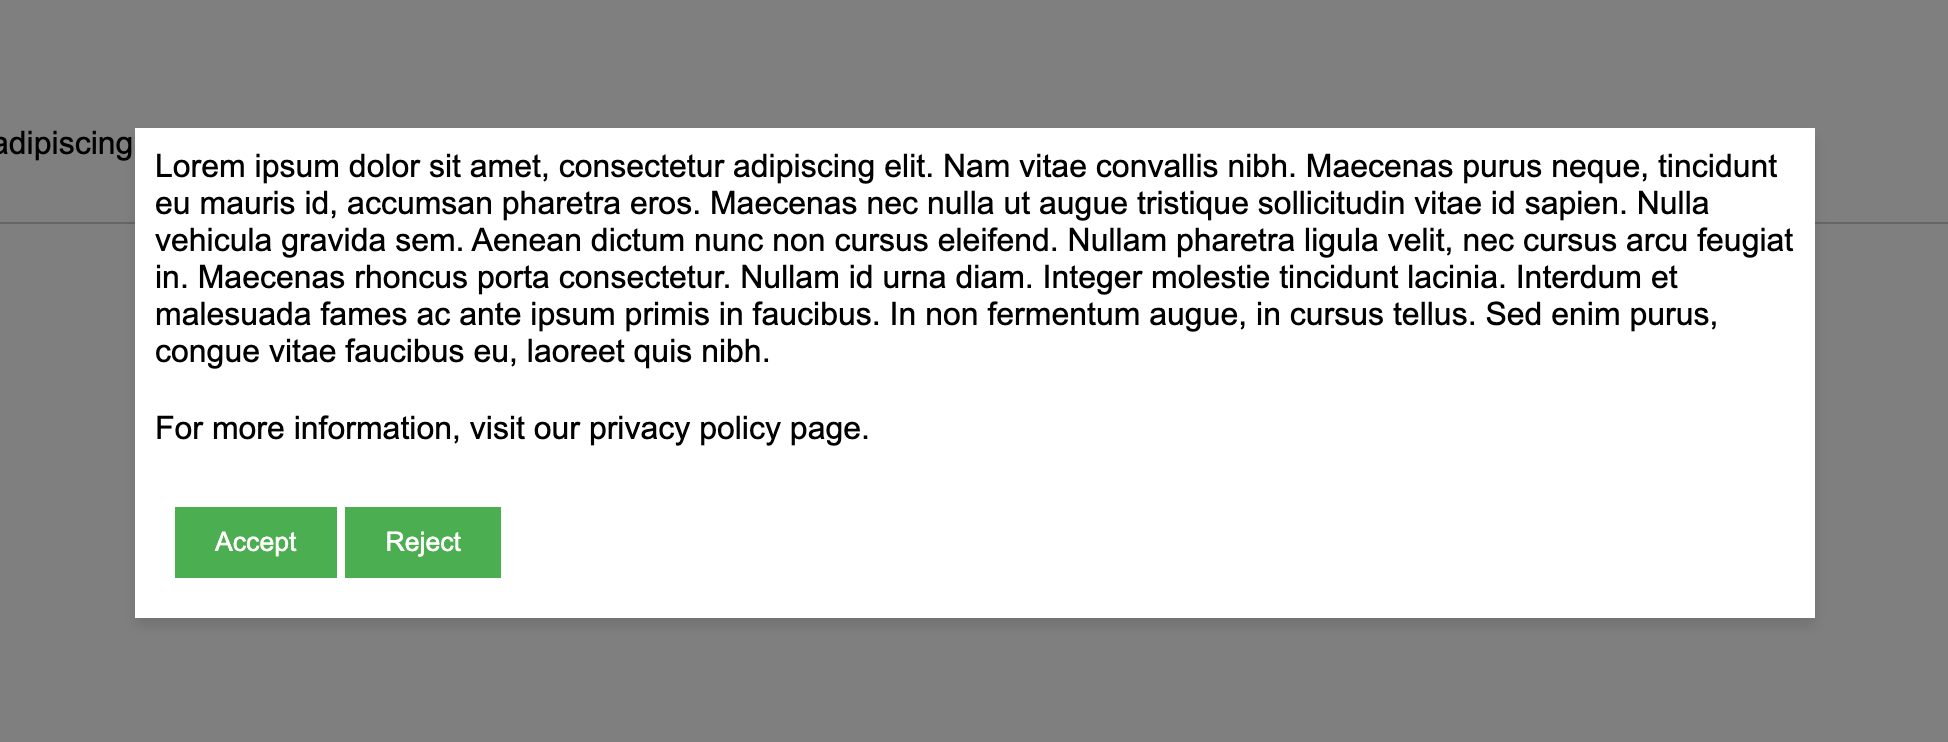
\includegraphics[width=1.0\linewidth]{media/screenshot_unselected.png}
	\end{minipage}\hfill
	\begin{minipage}{0.48\textwidth}
		\centering
		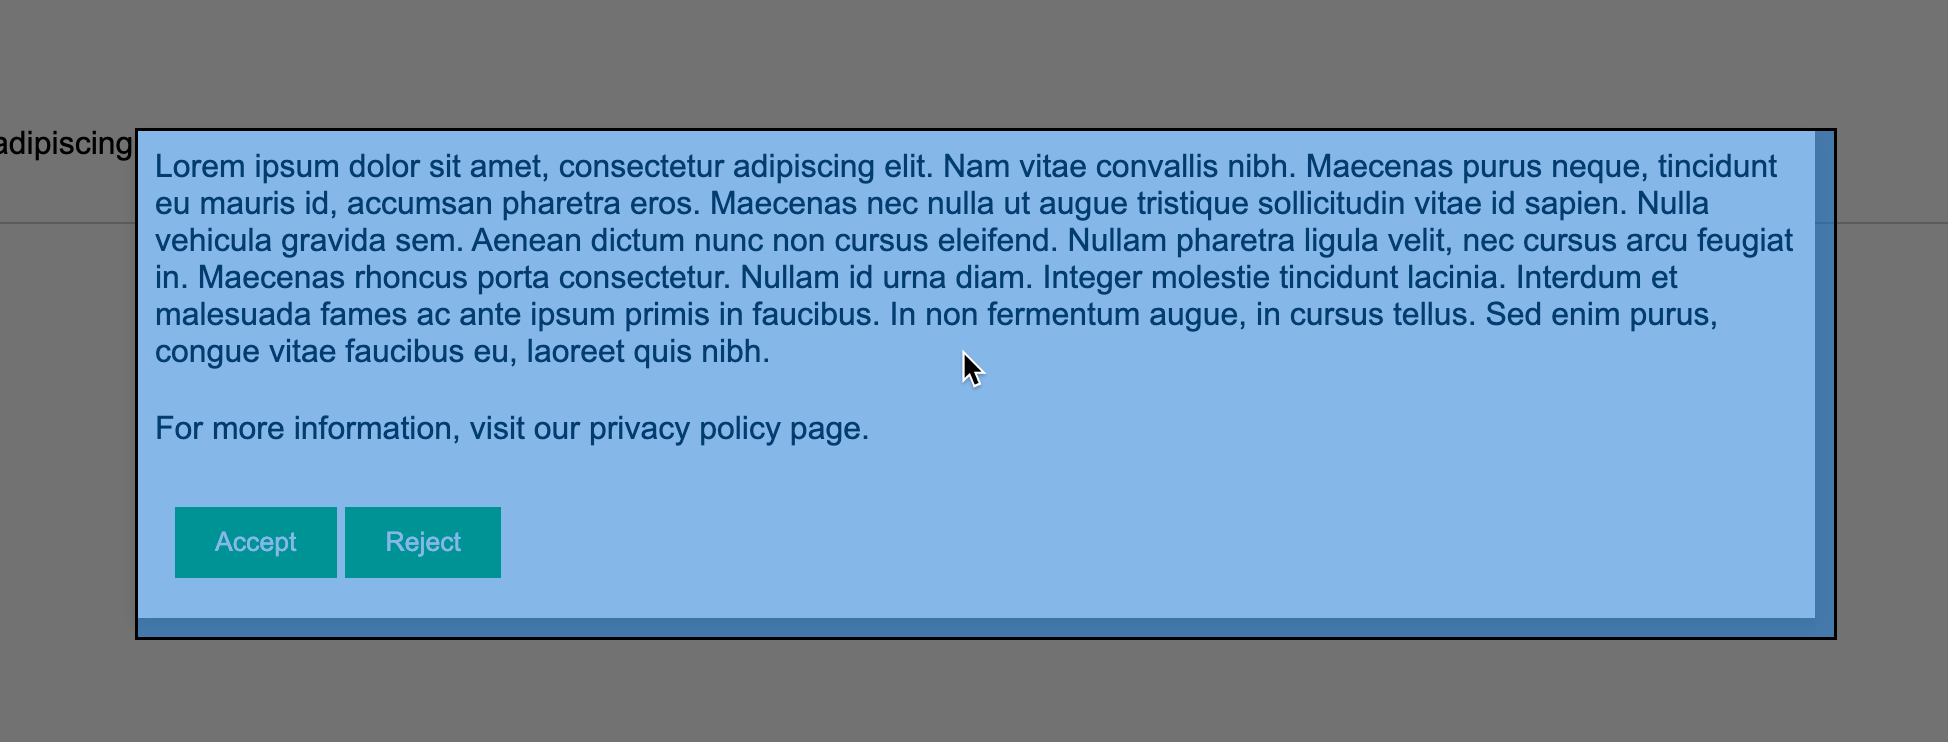
\includegraphics[width=1.0\linewidth]{media/screenshot_selected.png}      
	\end{minipage}
	\caption{Manual notice selection.}
	\label{fig:screenshot-selection}
\end{figure}

The picker is implemented as a \emph{content script}. 
As explained in \cref{subsec:content-scripts}, content scripts are JavaScript programs that can interact with the web page.

The activated picker tool listens for cursor movement by the user. 
On movement, it reads the coordinates of the cursor and determines the HTML element at that position.
The picker changes the styling of the determined element to provide visual feedback.
CookieAudit needs users to select the element corresponding to the complete cookie notice. 
Occasionally, the desired element is only a container whose area is filled out by the children (see \cref{fig:notice-fillout}).
In this case, every click inside the notice will select a child element rather than the entire notice container. 
Therefore, users won't be able to select the whole notice by simply hovering the cursor.
As a solution, we implement a context menu that appears after the user has clicked on an element.
With the menu, the user can traverse up the DOM tree to the element containing the whole cookie notice.
In the end, the selection can be confirmed via the context menu.


\begin{figure}
	\centering
	\begin{minipage}{0.48\textwidth}
		\centering
		\begin{tikzpicture}[]
			% Outer box
			\draw [thick] (0,0) rectangle (4,-3);
			
			% Child boxes
			\draw [fill=green!10] (0,0) rectangle (4,-0.7) node[midway, text=green!50!black] {Child 1};
			\draw [fill=orange!10] (0,-0.7) rectangle (4,-2.3) node[midway, text=orange] {Child 2};
			\draw [fill=purple!10] (0,-2.3) rectangle (4,-3) node[midway, text=purple] {Child 3};
		\end{tikzpicture}
	\end{minipage}\hfill
	\begin{minipage}{0.48\textwidth}
		\centering
		\begin{tikzpicture}[]
			% Outer box
			\draw [thick] (0,0) rectangle (4,-3);
			
			% Child boxes
			\draw [fill=green!10] (0.2,-0.2) rectangle (3.8,-0.8) node[midway, text=green!50!black] {Child 1};
			\draw [fill=orange!10] (0.2,-0.8) rectangle (3.8,-2) node[midway, text=orange] {Child 2};
			\draw [fill=purple!10] (0.2,-2) rectangle (3.8,-2.6) node[midway, text=purple] {Child 3};
		\end{tikzpicture}     
	\end{minipage}
	\caption{Any location in the left notice will map to one of the children. Only the white area in the right notice will be mapped to the whole notice.}
	\label{fig:notice-fillout}
\end{figure}

The complexity and variety of both HTML and JavaScript implementation details results in many possible ways of implementing cookie notices.
Because of this, we had to handle several edge cases which we encountered during the manual testing of CookieAudit.
Next, we will present our solutions.

\subsubsection{Inline Frame}
An inline frame (\texttt{iframe}) allows developers to embed another HTML context by specifying an external web address~\cite{iframeMdn}.
Some websites implement cookie notices with an \texttt{iframe} that refers to a Consent Management Platform.
To enable users to select the cookie notice, we inject the \emph{picker tool} content script not only into the original web page, but also into all \texttt{iframe} elements.

\subsubsection{Shadow DOM}
A shadow DOM separates the elements inside of it from the influence of the main document's JavaScript and CSS~\cite{shadowDomMdn}.
Some developers use this feature to integrate cookie notices into their web page.
This encapsulation prevents our picker content script from directly accessing the cookie notice elements. 
To address this, we implement a solution during user notice selection.
As described before, we continuously query for the element that is located at the user's cursor coordinates.
When a user hovers over an element within a shadow DOM, this query will return the root of the shadow DOM (\emph{shadow root}). 
We then check if the element is indeed a shadow root by reading the \texttt{shadowRoot} property of the HTML element.
If so, we explicitly enter the shadow DOM context and query for the element at the user's cursor coordinates once again. 

\subsubsection{Dialog Element}
The \texttt{dialog} element is an HTML element that can be used to build dialog boxes such as cookie notices.
When opened, it is displayed above the other elements of the website and covers elements with arbitrary \texttt{z-index} values. 
Multiple \texttt{dialog} elements are stacked based on their opening order, with the most recent dialog displayed on top.
If used to display a cookie notice, a dialog element would also hide our picker tool context menu.
Therefore, we have implemented the menu with a \texttt{dialog} element.
By opening our dialog after the cookie notice renders, we ensure that the menu will be visible and accessible to CookieAudit users.

\section{Cookie Notice Analysis}
For the analysis of a selected cookie notice, we rely on the extraction and classification functionality developed by Bouhoula et al.~\cite{bouhoula2023automated}.
We use their NLP models to detect declared cookie purposes in the cookie notice text and to classify interactive elements of the notice for later interaction.
In case of a detected \emph{Settings} button, we additionally analyze the corresponding settings page.

\subsection{Extraction} \label{subsec:extraction}
To extract the cookie notice text, we iterate through all visible elements inside the notice and concatenate their text content.
For nested elements, which are common in HTML's tree-like structure, we recursively repeat this process.

To enable automated interaction with cookie notices, CookieAudit needs to identify all clickable elements.
We use the criteria proposed by Bouhoula et al.~\cite{bouhoula2023automated}.
First, we consider only elements of type \texttt{div}, \texttt{span}, \texttt{a}, \texttt{button} or \texttt{input} that fulfill one of the following criteria: 
has the accessibility (ARIA) role \texttt{button}, 
has the attribute \texttt{onclick} or
has a non-negative \texttt{tabindex}.
Furthermore, we consider elements that change the mouse to a pointer when hovered over.
The last criterion was added based on manual testing, as it captured some interactive elements missed by the other rules in rare cases.

\subsection{Classification}
According to the GDPR, users need to be able to provide informed and explicit consent.
Therefore, a cookie notice needs to (i) declare the purposes of its data collection and processing and (ii) provide interactive elements for the user to express his explicit consent (\emph{Accept} button) or rejection (\emph{Reject} button).
Bouhoula et al.~\cite{bouhoula2023automated} trained the two BERT models~\cite{devlin2018bert}, the \emph{purpose detection} model and the \emph{interactive elements} model, for both classification problems.
Next, we will explain how we integrate and use the models.

\subsubsection{Purpose detection model}
The purpose detection model classifies sentences into either Purposes for Analytics/Advertising (profiling, advertising, custom content, analytics, and social media features) or Other Purposes (essential functionalities, offering service, and website/UX enhancement).
Because the models only work on English input, CookieAudit first translates (if necessary) the cookie notice text using a public translation API.
The translated text is then classified with the browser library Transformer.js~\cite{huggingface2023transformers} which makes it possible to efficiently\footnote{
We have found the average time of a sentence classification to be 209ms. 
To determine this, we benchmarked the classification of 1187 sentences using the purpose detection model in a Chrome extension using Transformers.js.
The sentences are from a dataset by Santos et al.~\cite{santos2021cookie} and were also used to train the purpose detection model.
The benchmark was done on a MacBook Pro with an Intel i5 7267U 3.10GHz CPU and 16 GB memory while no other user space programs were running.
} run BERT models on the client.

\subsubsection{Interactive elements model}
CookieAudit has to understand the functionality of the interactive cookie notice elements to be able to automatically interact with them.
The interactive elements model by Bouhoula et al. classifies the texts of buttons as either accept, reject, close, save, settings and other.
Because it is also a BERT model we can run it, after a translation of the texts, equivalently to the purpose detection model.

\subsubsection{Cookie classification model}
We use the CookieBlock model by Bollinger et al.~\cite{bollinger2022automating} which classifies cookies into the four purposes \textsf{Necessary}, \textsf{Functional}, \textsf{Analytics}, and \textsf{Advertising}.
The model relies on features such as one-hot encoding of common cookie names and domains, the presence of specific data types, the cookie's expiry date and entropy, or the edit distance between cookie updates.
The ensemble model was trained on a dataset of cookies that were collected from crawling 27k websites which employed one of the CMPs: OneTrust, Cookiebot, or Termly.
These CMPs provide labels for individual cookies.

\subsection{Exploration}
Cookie notices can offer additional settings.
The settings may contain a declaration of cookie purposes, or interactive elements, e.g, to reject specific cookie categories or even all non-necessary cookies.
Therefore, CookieAudit needs to open and analyze the settings.

If a \emph{Settings} button is available in a cookie notice, clicking it may change the content of the current notice to display the settings, open a new settings notice or open a separate web page with the settings.
Similar to the approach implemented by Bouhoula et al.~\cite{bouhoula2023automated}, CookieAudit clicks on all interactive elements that were classified as \emph{Settings}.
If no interactive elements were classified as \emph{Settings}, CookieAudit alternatively uses three \emph{Other} elements. 
In particular, the \emph{Other} elements are sorted by their y-coordinates, such that elements that are located on the bottom of the cookie notice are used.
This simple heuristic is based on the observation that the \emph{Settings} button is often located at the bottom.
After the \emph{Settings} have been opened and identified, CookieAudit will again proceed as for the original cookie notice, retrieving and analyzing the text and interactive elements.
CookieAudit saves the elements of type \emph{Reject}, \emph{Close} and \emph{Save Settings} to the extension storage. The stored entries are pairs of selectors containing the \emph{Settings} element selector, and the second layer element selector.

Based on the work by Bouhoula et al.~\cite{bouhoula2023automated}, we implemented the detection and handling of the following three scenarios:

\subsubsection{New Cookie Notice}
The cookie notice settings can be displayed inside a new notice that appears, e.g., above the original cookie notice. 
CookieAudit detects this situation if one of the following criteria holds:

\begin{itemize} 
    \item a query for the cookie notice with the selector returns \texttt{null},
    \item the cookie notice is not visible anymore (e.g., if the notice has or inherits an \texttt{opacity} of 0, has or inherits the CSS \texttt{visibility} of hidden or collapse, or has an area of 1 pixel or less),
    \item the notice still exists and is visible, but \emph{neither} its text content nor the dimensions (height and width) have changed after the interactive element click, or
    \item the cookie notice is covered by another element. CookieAudit runs \texttt{elementFromPoint()} at the coordinates of the cookie notice center. If the returned element is not the notice or contained in the notice, we consider the notice covered.
\end{itemize}

To identify the settings element and start the analysis, CookieAudit activates the \emph{Cookie Notice Picker} (as described in \cref{subsec:user-aided-selection}) and lets the user manually select the settings notice.

\subsubsection{New Web Page}
CookieAudit stores the URL of the web page before the interactive element click and compares it to the URL of the web page after the click.
If it has changed, CookieAudit classifies the outcome as a new notice on a separate web page.
In this case, CookieAudit starts the cookie notice picker. 
The picker can be used to select both settings that are part of the normal flow of the web page, or displayed as a hovering dialog.
After the user selection and subsequent settings analysis, CookieAudit returns to the URL where the scan was started.

\subsubsection{Same Cookie Notice}
If neither the criteria of a \emph{New Cookie Notice} nor \emph{New Web Page} apply, CookieAudit assumes the settings to be now contained in the original cookie notice.
This effectively means that the original cookie notice is still visible, the contents, or dimensions have changed and the URL of the web page is still the same.
CookieAudit directly starts the settings notice analysis without any user interaction.

\section{Dark Pattern Detection}
Deceptive user interface designs that aim to manipulate user behavior and choices can be used in cookie notices.
Nouwens et al. have found such dark patterns in cookie notices to significantly influence user behavior towards providing consent~\cite{nouwens2020dark}.
Because some dark patterns could be considered forbidden under the GDPR in specific jurisdictions~\cite{gray2021dark}, we include detection of dark patterns as part of the CookieAudit extension.
Specifically, we consider the same three characteristics as Bouhoula et al.~\cite{bouhoula2023automated} in our analysis: \enquote{No reject button}, \enquote{Interface interference}, and \enquote{Forced action}.
Next, we will describe how CookieAudit detects \enquote{Interface interference} and \enquote{Forced action}.

\subsection{Interface interference}
Stöver et al.~\cite{stover2022website} define interface interference as ~\enquote{design (color, font, size) of the buttons for accepting and rejecting cookies are not equivalent.}
To find cases of interface interference, CookieAudit compares design characteristics of \emph{positive consent options} (accept button) with all \emph{negative consent options} (reject, save, and close buttons).

Typography differences of buttons can be detected by comparing the CSS attributes of the HTML elements, e.g., \texttt{font-size}.
The dominant color of a button is influenced by many potential factors, e.g., transparency of a button, background images, or gradients.
Therefore, CookieAudit captures a screenshot of the visible web page using the WebExtensions API and analyzes it to reliably determine the dominant colors of the buttons
After the screenshot is taken, the extension crops the image for all buttons according to their coordinates and determines the dominant color for each consent option with a k-means analysis.
Once all dominant colors have been identified, CookieAudit calculates the color differences between the positive and negative consent options.
The Euclidean distance over RGB (red, green, blue) color tuples would not accurately represent the perception of humans. 
Instead, the extension uses the $\Delta E_{ITP}$ color difference metric~\cite{ITURBT2124} which is based on a uniform color space, that is, \enquote{a color space in which equivalent numerical differences represent equivalent visual differences, regardless of location within the color space}~\cite{x_rite2024color}.
The $\Delta E_{ITP}$ metric is defined such that a difference below 1 is not noticeable for the human eye. We consider two colors to be mismatched when their $\Delta E_{ITP}$ difference is higher than 25.

\subsection{Forced action}
Stöver et al.~\cite{stover2022website} define \enquote{Forced action} as the requirement for a user to first engage with a cookie notice before entering the website.
In its most extreme form, this would be a \enquote{cookie wall} which forces the user to first accept all cookies and tracking technologies~\cite{bouhoula2023automated}.
Gray et al.~\cite{gray2021dark} considers \enquote{Forced action} to be a dark pattern.
Bouhoula et al.~\cite{bouhoula2023automated} argue that such a design is not necessarily intentional deception, as it may even raise the privacy awareness of users, according to Bakos et al.~\cite{bakos2014fineprint}.
CookieAudit will report any detected \enquote{Forced Action} as a dark pattern.

\enquote{Forced Action} prevents the user to interact with the rest of the website, e.g., clicking on links outside the cookie notice.
First, CookieAudit samples 10 links from the website, which are located in the viewport and are visible according to their CSS attributes.
Because the cookie notice body may cover some links but still allow most website interaction,\footnote{
For example, a cookie notice can cover the navigation header while the body of the website is still accessible.
} CookieAudit selects, if possible, links that are not hidden by the cookie notice body.
Next, CookieAudit will determine whether the links are unresponsive while the cookie notice is open, but clickable after CookieAudit has provided positive consent, i.e., clicked the \textsf{Accept} button.
For a browser extension, there is no general method to determine if a link is clickable by the user. 
Instead, CookieAudit will approximate the \enquote{clickability} by determining whether a link is covered by another element, e.g., by a semi-transparent overlay that blocks user clicks.
CookieAudit reports forced action if at least one link which is covered before any consent is given,\footnote{All default counts and thresholds can be configured by the user.}
is accessible after the cookie notice is closed by CookieAudit.

\section{Managing Page Loads and Changes}
In the course of a website scan, CookieAudit repeatedly reloads the website and visits multiple subpages.
The extension always needs to wait until all relevant content has been loaded, e.g., CookieAudit can only start analyzing the text and links in the cookie notice once all of them have been rendered in the browser.
CookieAudit uses the WebExtensions API \texttt{tabs.onUpdated} to determine when a website is fully loaded and rendered.
The \texttt{tabs.onUpdated} event object informs a browser extension about the loading state of the initial HTML document and its immediate resources (CSS, JavaScript, and hard-coded images).
However, the event object does not inform CookieAudit when websites dynamically add content, which is also possible after the initial HTML document is loaded.
The loading state, that CookieAudit receives from the WebExtensions API, is also indicated in the Chrome browser interface with a loading icon.
\cref{fig:screen-website-loading} shows a website dynamically adding a CMP-based cookie notice after Chrome considers the website to be loaded.
Therefore, CookieAudit must detect dynamic changes in a website's content after the initial HTML document has finished loading.

CookieAudit needs to watch the whole DOM subtree rooted in the document body for changes because any update could be relevant for the website analysis.
The \texttt{MutationObserver} interface, which is implemented in all major browsers, can be used to efficiently watch for mutations in a website's DOM tree~\cite{whatwg2024interface}.
We configure the \texttt{MutationObserver} to monitor the document body subtree for additions or removals of child elements.
We consider the website to be loaded when no new changes are observed for two seconds.
Because some websites continuously make dynamic DOM changes, e.g., loading and adding new posts to a timeline, we add a general timeout of ten seconds.
During manual testing, we observed the timeout of ten seconds to be effective.
In all cases where it was reached because of continuous DOM changes, the websites had already finished loading all required elements\footnote{
Depending on the stage of the scan, not only the cookie notice is required.
For example, the navigation header is needed to find subpages of the website during the consent options testing.
} for CookieAudit.

\begin{figure}[htbp]
    \centering
    \begin{subfigure}[b]{0.48\textwidth}
        \centering
        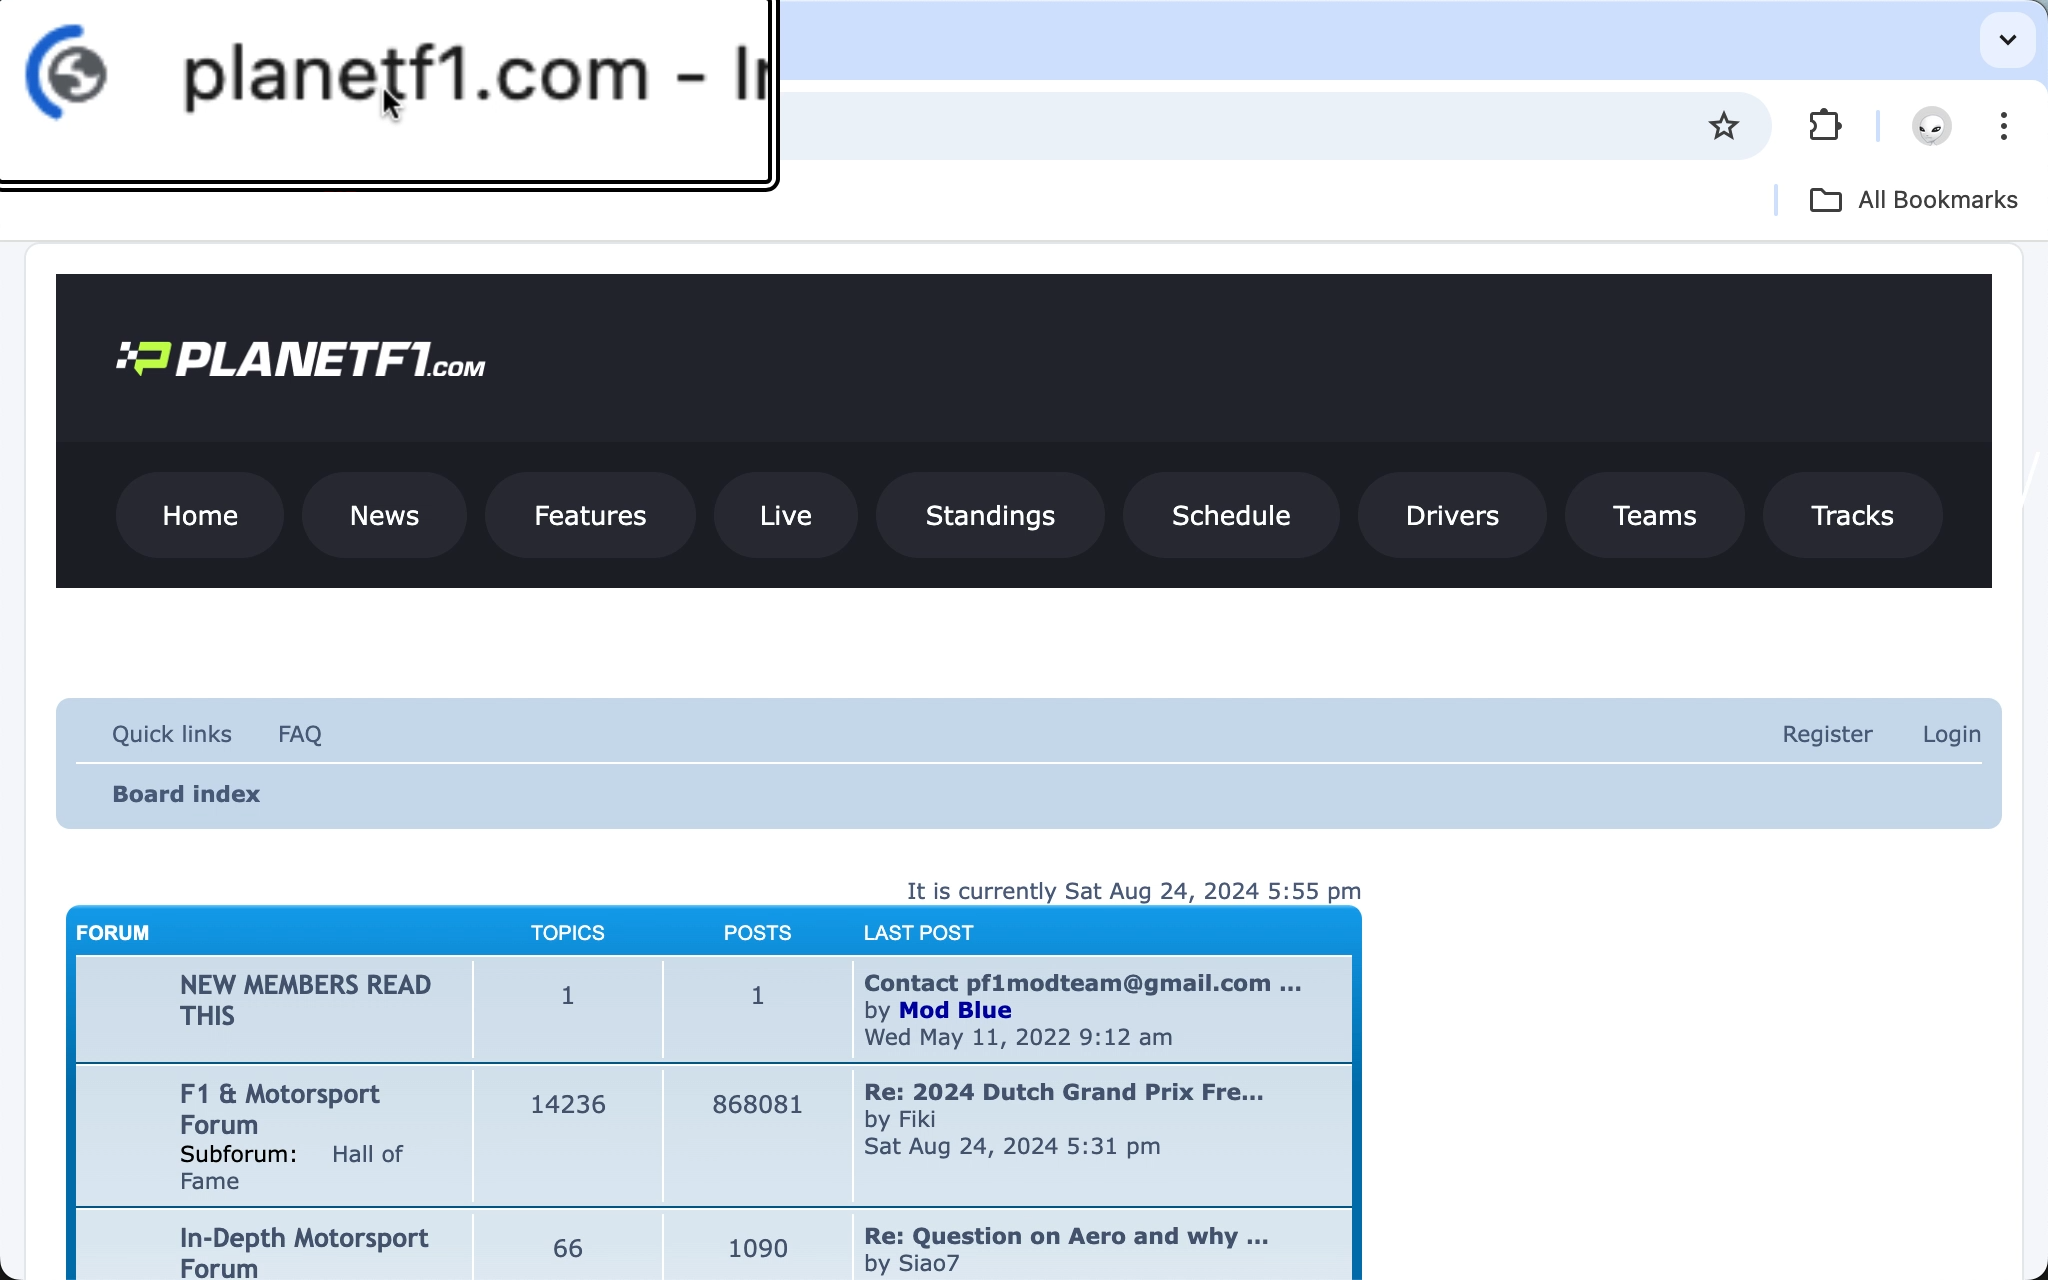
\includegraphics[width=\textwidth]{media/screen_load.png}
        \caption{The spinning loader indicates that the website is loading the initial HTML document.}
        \label{fig:screen-load}
    \end{subfigure}
    
    \vspace{1em}
    
    \begin{subfigure}[b]{0.48\textwidth}
        \centering
        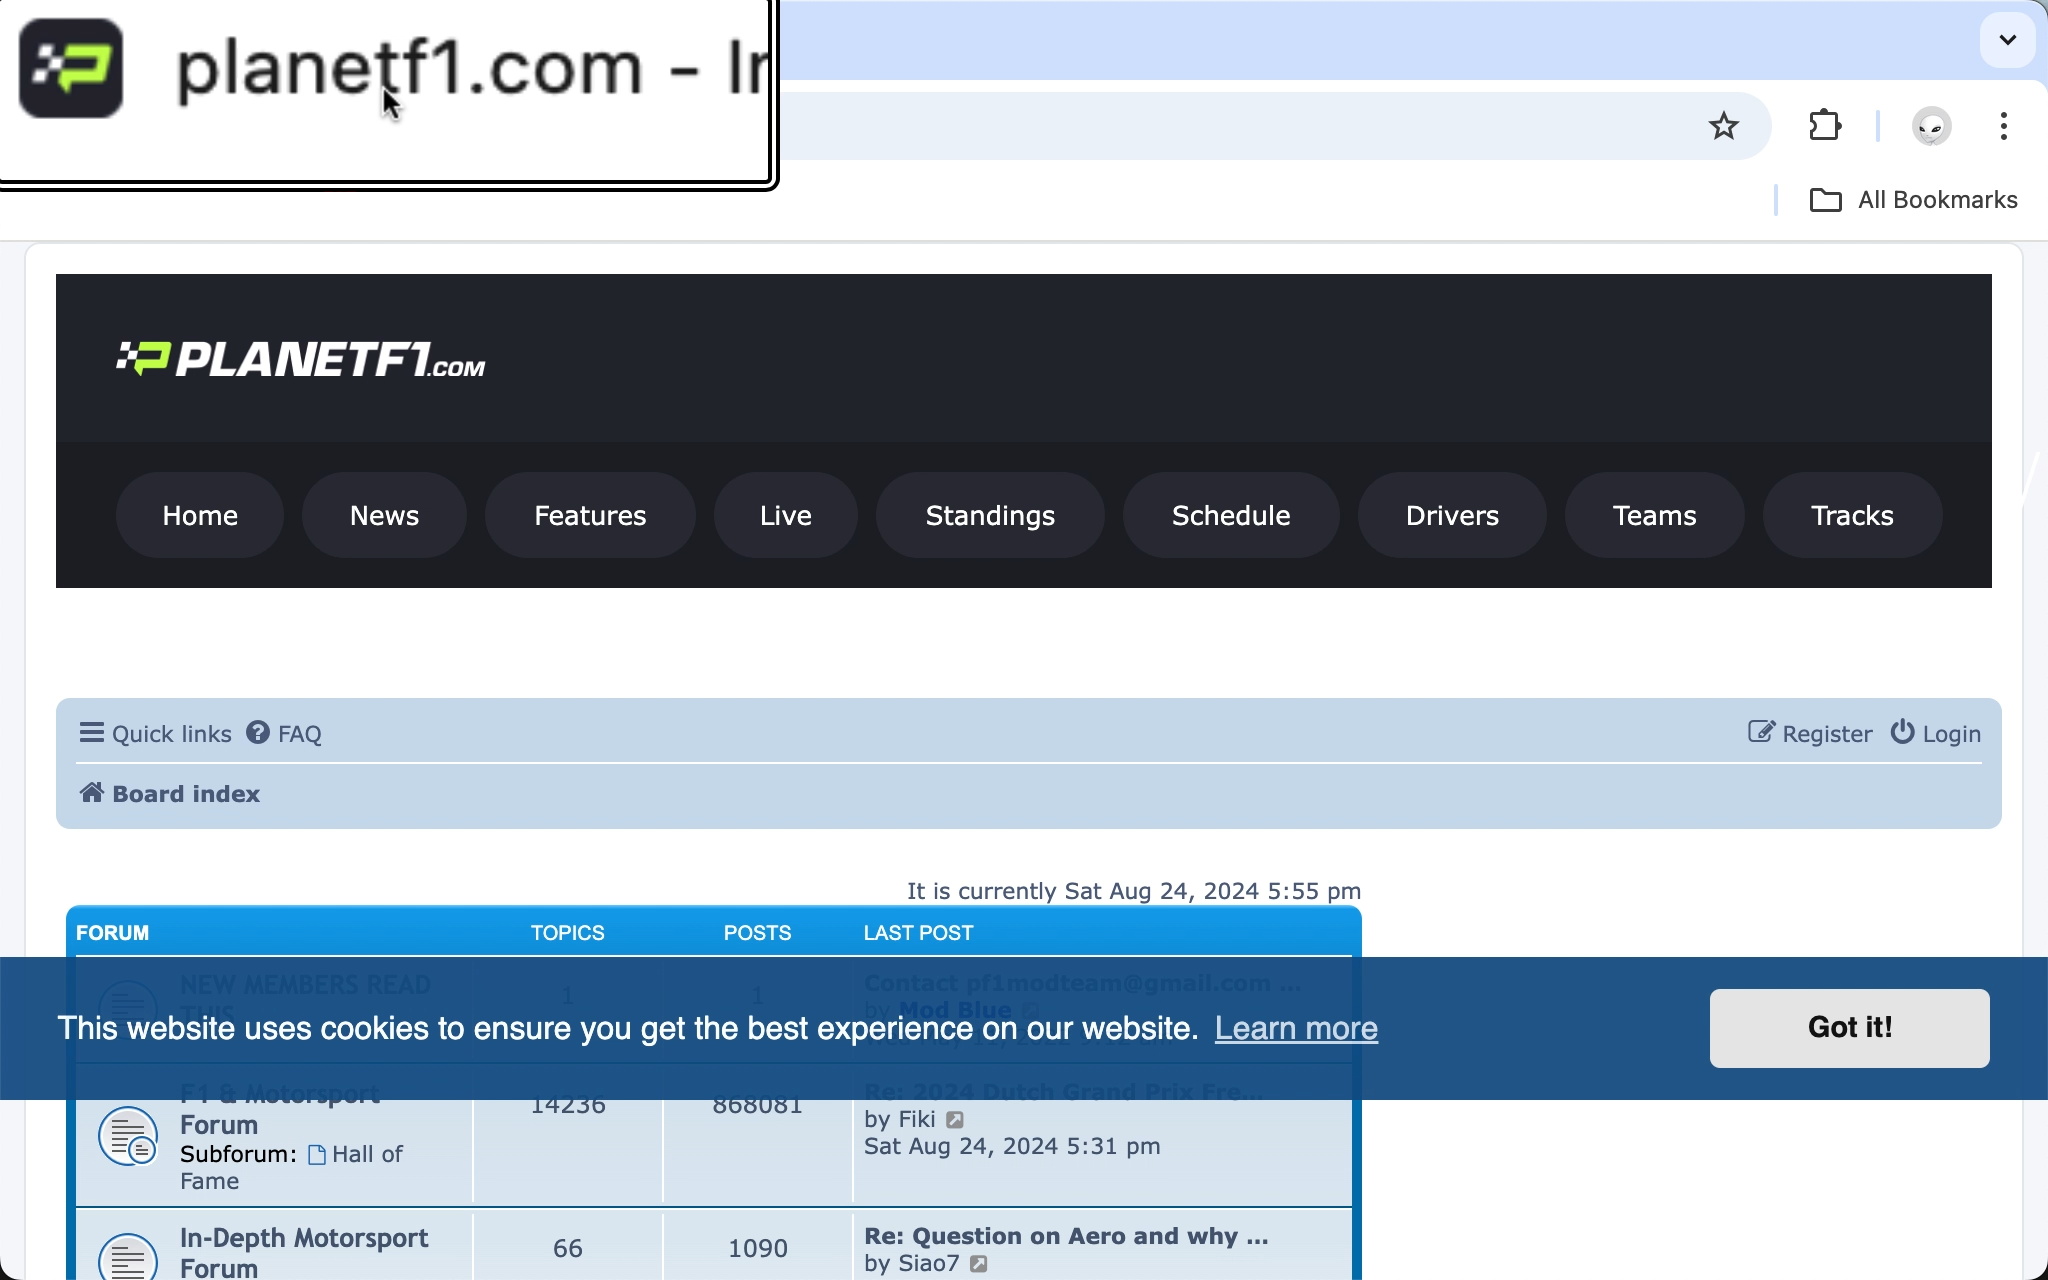
\includegraphics[width=\textwidth]{media/screen_loaded.png}
        \caption{The initial HTML document has been loaded.}
        \label{fig:screen-loaded}
    \end{subfigure}
    \hfill
    \begin{subfigure}[b]{0.48\textwidth}
        \centering
        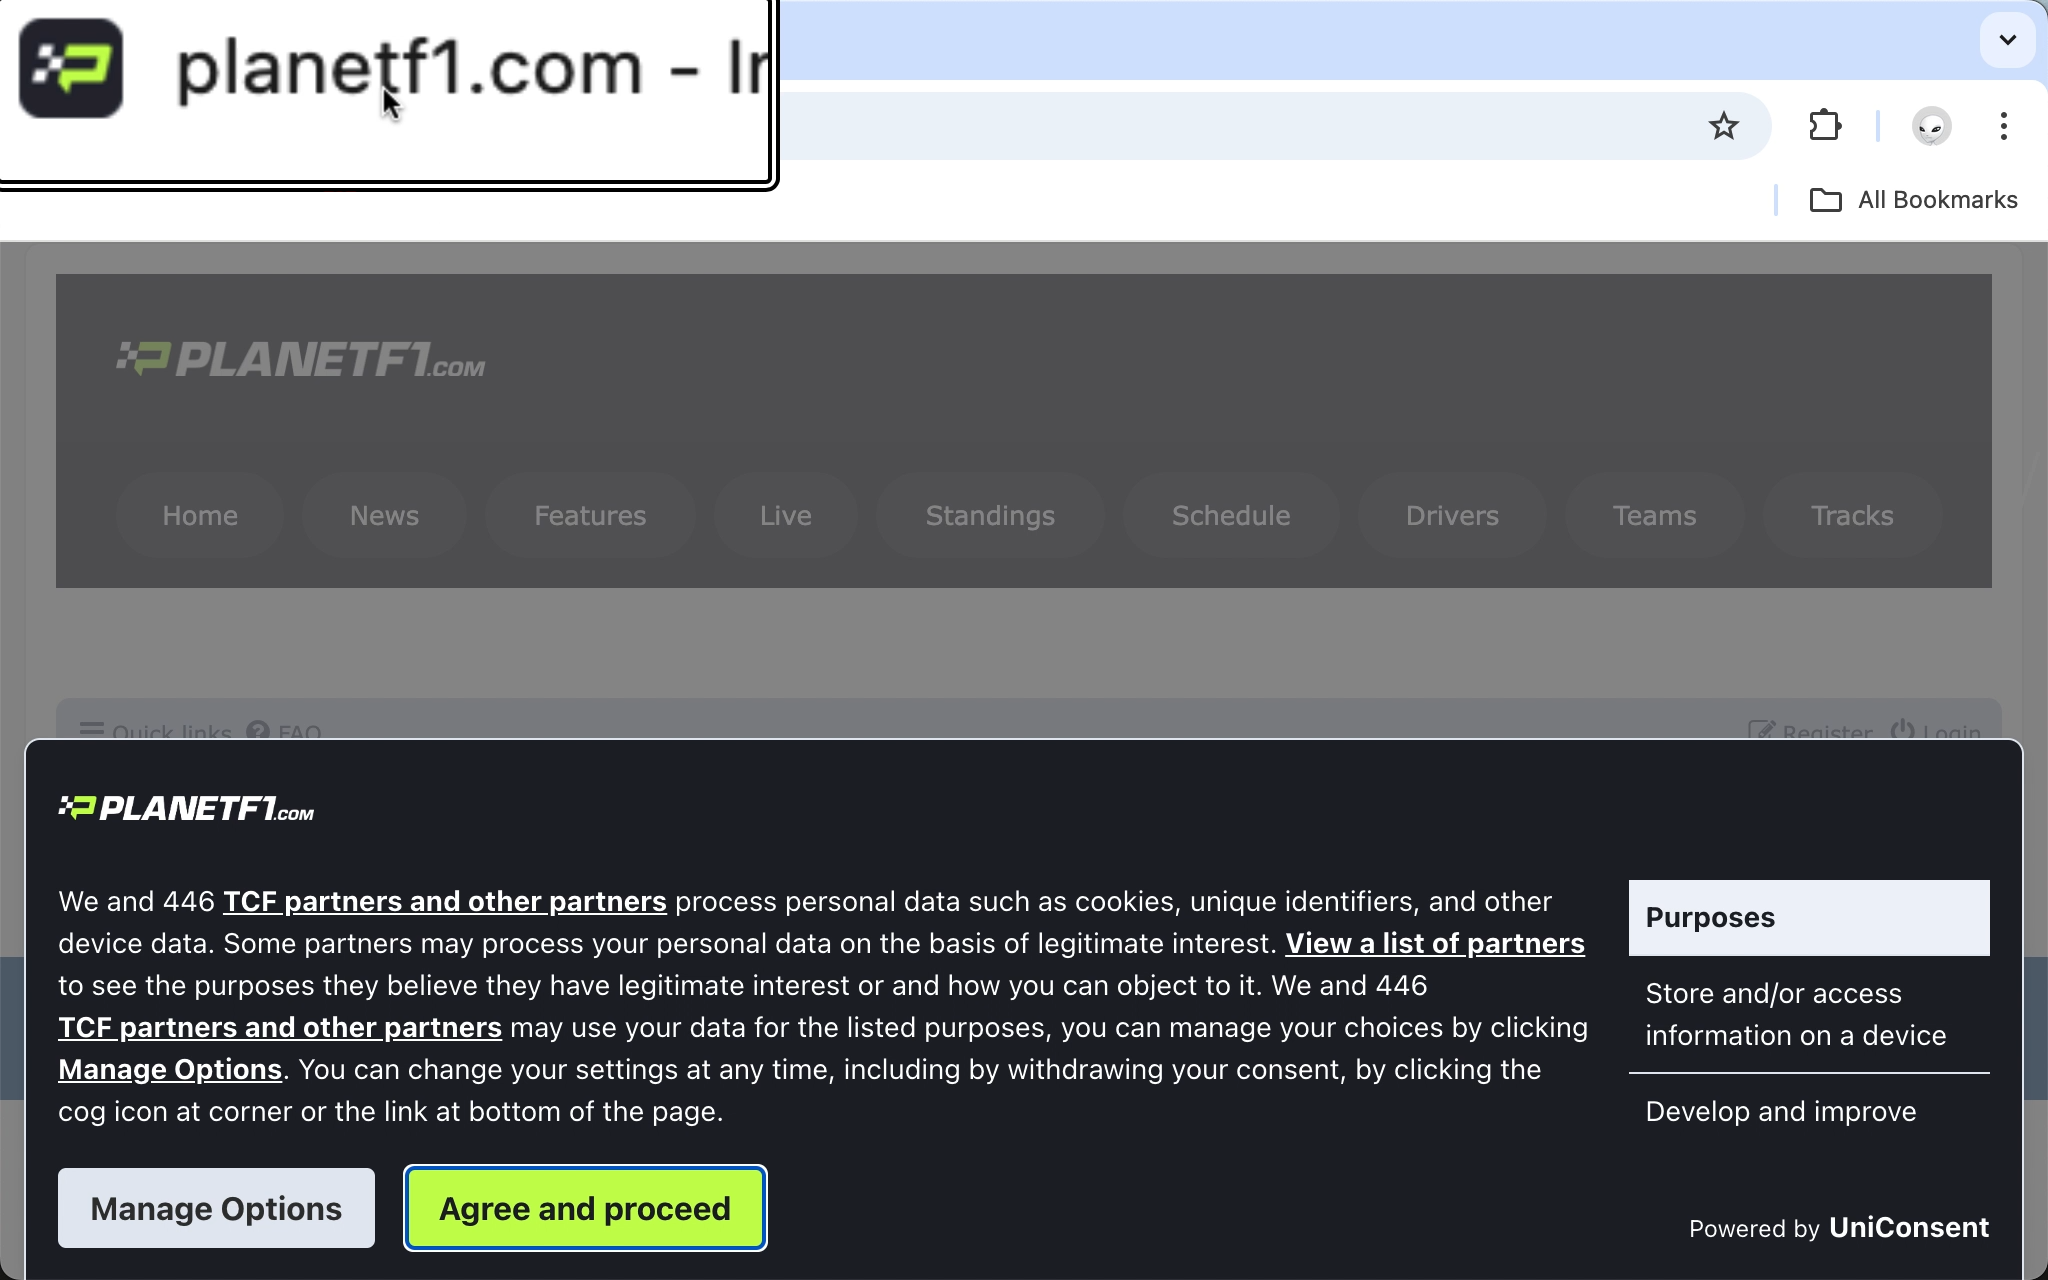
\includegraphics[width=\textwidth]{media/screen_loaded-dynamic.png}
        \caption{Dynamic changes are not indicated by a change in the loading state.}
        \label{fig:screen-loaded-dynamic}
    \end{subfigure}
    \caption{Website loading sequence: initial page load, HTML rendering completion, and optional dynamic content update.}
    \label{fig:screen-website-loading}
\end{figure}

\section{Report Creation}
After the scan, CookieAudit compiles two reports summarizing the collected data and analysis.
The first report is a PDF file created using the JavaScript-based pdfmake library.
Pdfmake is a document generation library for the browser that enables the convenient styling and layout of document contents, table layouts with header repetition across page breaks, and automatic download functionality that doesn't require the user to manually "print" a report document.

To generate the machine-readable JSON report, CookieAudit collects all relevant data in a JavaScript object, converts it into a string and writes it into a .json text file.
The conversion is straightforward because JSON is derived from JavaScript objects.
The JSON report contains more data that was collected by CookieAudit, e.g., the complete cookies that resulted in violations.

\begin{figure}
	\centering
	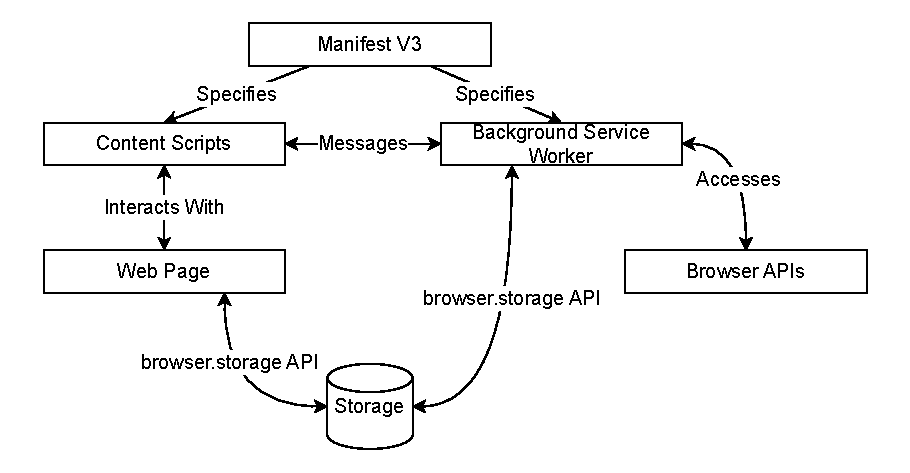
\includegraphics[width=\textwidth]{media/browser-extension-architecture.drawio.pdf}
    \caption{The general architecture of a manifest version 3 browser extension.}
    \label{fig:extension-architecture}
\end{figure}

\chapter{Testing on Websites}

\section{Creating a Set of Websites}

We will create two distinct sets of websites to test and evaluate the CookieAudit browser extension. 
The websites will be a random sample based on the dataset of Bouhoula et al.~\cite{bouhoula2023automated}. 
The first set will contain 50 websites from 5 countries (France, Germany, Poland, Ireland, and the USA).
We will sample websites of different levels of popularity from the Chrome User Experience report~\cite{chrome2024crux}.
Specifically, we will cover web pages from the CrUX ranks\footnote{For example, the CrUX rank 1k contains the 1000 most popular web pages of a given country.} 1k, 5k, 10k, 100k and 500k.
CookieAudit has to work with common Consent Management Providers to be a practical tool.
The second set will therefore contain 20 websites, with each using one of the 20 most common CMPs. 
After manually running the CookieAudit browser extension on the websites, we will compare the results with the corresponding findings of Bouhoula et al.~\cite{bouhoula2023automated}.

% \backmatter  % Template v2 fixes: this just breaks things

% Template v2 fixes: Bibliography belongs before appendix
\printbibliography

\appendix
\chapter{Dummy Appendix}

You can defer lengthy calculations that would otherwise only interrupt
the flow of your thesis to an appendix.


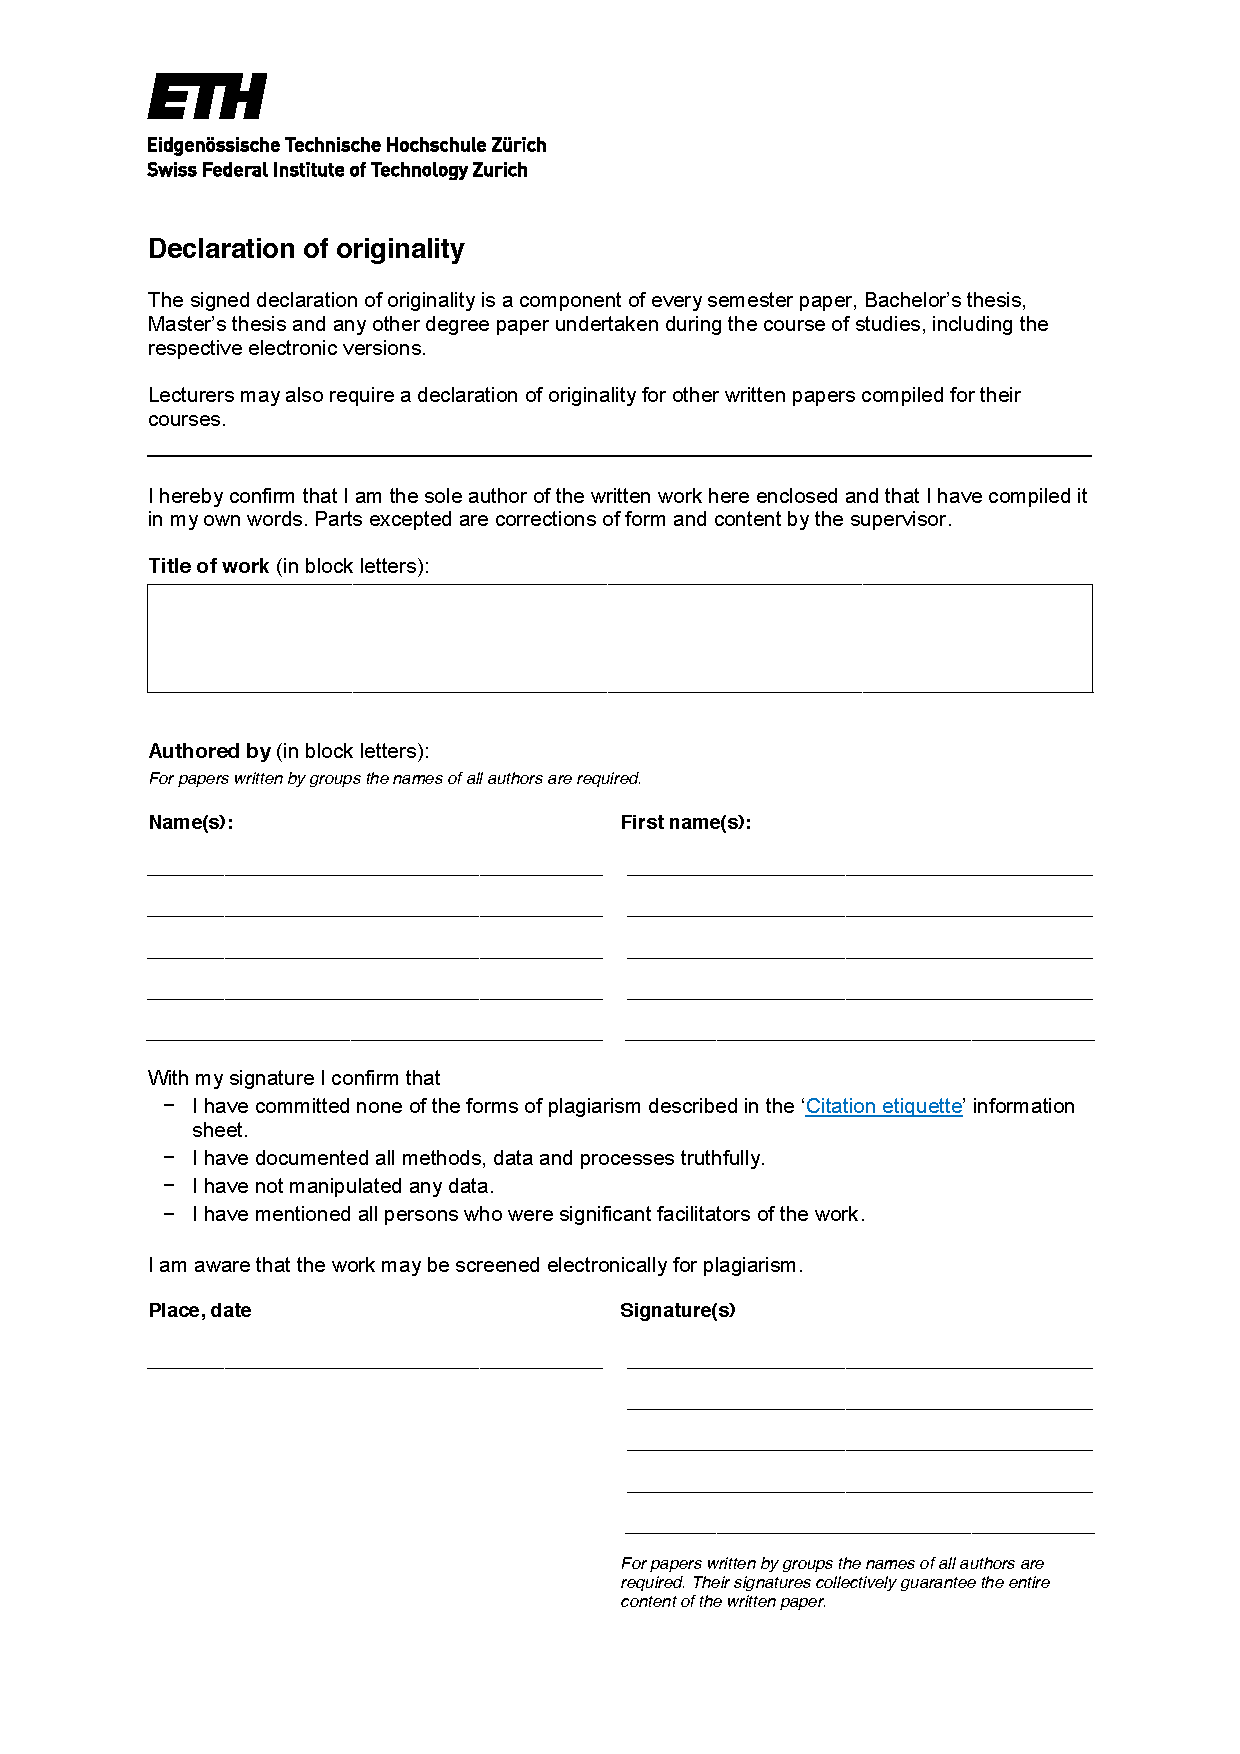
\includepdf[pages={-}]{eth-template/declaration-originality.pdf}

\end{document}
